
\documentclass{article}
\usepackage{neurips_2023}
\usepackage[utf8]{inputenc}
\usepackage{geometry}
\usepackage{fancyhdr}
\usepackage{amsmath}
\usepackage{amssymb}
\usepackage{xspace}
\usepackage{bm}
\usepackage{xcolor}
\usepackage[colorlinks,linkcolor=blue]{hyperref}
\usepackage{graphicx}
\usepackage{url}
\usepackage{float}
\usepackage{subcaption}
\usepackage{listings}
\usepackage{enumitem}
\usepackage{booktabs}
\usepackage{multirow}
\usepackage{hyperref}
\usepackage{cleveref}


\makeatletter
\DeclareRobustCommand\onedot{\futurelet\@let@token\@onedot}
\def\@onedot{\ifx\@let@token.\else.\null\fi\xspace}
\def\iid{\emph{i.i.d}\onedot} \def\IID{\emph{I.I.D}\onedot}
\def\eg{\emph{e.g}\onedot} \def\Eg{\emph{E.g}\onedot}
\def\ie{\emph{i.e}\onedot} \def\Ie{\emph{I.e}\onedot}
\def\cf{\emph{c.f}\onedot} \def\Cf{\emph{C.f}\onedot}
\def\etc{\emph{etc}\onedot} \def\vs{\emph{vs}\onedot}
\def\wrt{w.r.t\onedot} \def\dof{d.o.f\onedot}
\def\aka{\emph{a.k.a}\onedot}
\def\etal{\emph{et al}\onedot}
\makeatother

\newcommand{\important}[1]{{\color{blue}{\bf\sf #1}}}

\title{CPEN455 Final Project: PixelCNN++G}
\author{
  Guan Zheng Huang \\
  CPEN 455\\
  UBC\\
}


\begin{document}

\pagestyle{fancy}
\fancyhead{} 
\fancyhead[L]{\textbf{UBC CPEN455 2023 Winter Term 2}}
\fancyhead[R]{\textbf{Final Project: PixelCNN++G}}

\maketitle
\thispagestyle{fancy}
\begin{abstract}
    This work introduces PixelCNN++G, an image generation model derived from the PixelCNN++ architecture [1]. PixelCNN++G, a conditional generation model, can also be used for image classification. We demonstrate the capabilities of this modification by training the model on the CPEN450 dataset, categorizing images into four classes.
\end{abstract}

\section{Model}

\subsection{PixelCNN++G Improvements}

    \subsubsection{Data Preprocessing:}
    \begin{itemize}
        \item PixelCNN++ is sensitive to image orientation, which can hinder its ability to accurately recognize object orientations. To mitigate this, we horizontally flip the images randomly during training, which not only helps the model become invariant to direction but also effectively doubles the training dataset, enhancing the model's generalization capabilities.
        \item We also rotate the images randomly within a range of -10 to +10 degrees. This helps the model to better learn object orientations with minimal influence from image directionality.
        \item Further, we employ new data augmentation techniques during the fine-tuning stage, such as color jittering and random cropping, to expose the model to more varied data, which is crucial in the fine-tuning process. 
    \end{itemize}

    \subsubsection{Conditional Model:}
    \begin{itemize}
        \item The model is conditioned on image class labels, which is represented as one-hot encoding.
        \item Within the \texttt{gated\_resnet} function, we introduced two additional layers (\texttt{weight\_a} and \texttt{weight\_b}), each multiplicatively interacting with the input label before adding to the resultant parameters (\texttt{a}, \texttt{b}) post-convolution. This approach enables the model to learn class-specific features at each layer effectively. To illustrate this, a simplified diagram of PixelCNN++G is presented in Figure \ref{fig:o-dia}. It is important to note that this diagram omits detailed features such as shifting and masking; it focuses on demonstrating the influence of the weighting mechanism.
    \end{itemize}

    \subsubsection{Classification Layer:}
    \begin{itemize}
        \item We implemented a classification layer using a modified per-image loss function. By evaluating each image across all potential labels and choosing the label that yields the lowest loss, the model predicts the image's label. This approach, conceptually similar to \texttt{argmin(softmax(logits))}, avoids the pitfalls of floating-point precision errors found in the softmax approach, which occasionally lead to incorrect predictions.
    \end{itemize}

    \subsubsection{Finetuning Pipeline:}
    \begin{itemize}
        \item A new fine-tuning pipeline has been developed to enhance the model's performance on specific classes or across all classes with a reduced learning rate. This pipeline can incorporate a validation set for additional data analysis; however, subsequent validation on this portion might skew results. This process was not used to produce the final PixelCNN++G checkpoint as the base model performed best, demonstrating efficacy in addressing class imbalance issues observed in other models. A detailed review of this process and the result comparison is available in the appendix under section \ref{train}.
    \end{itemize}

\begin{figure}
    \centering
    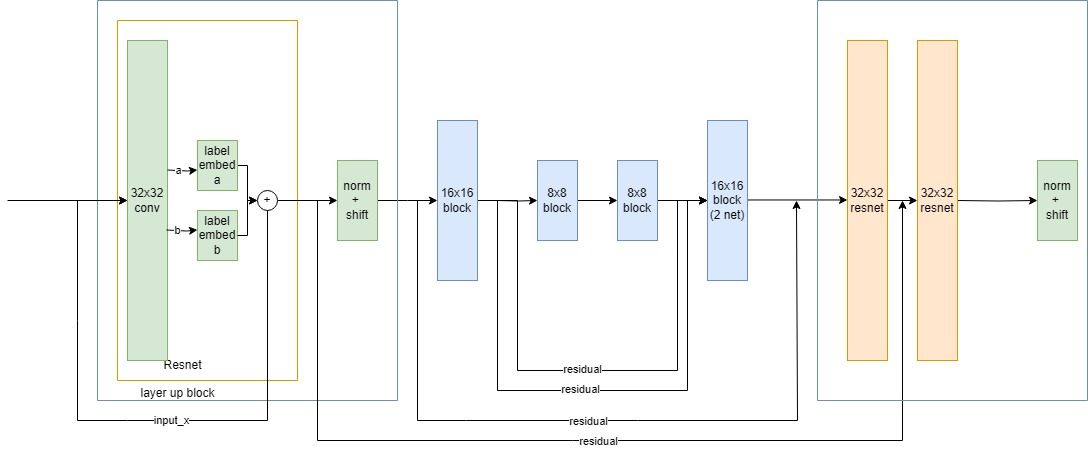
\includegraphics[width=1.0\textwidth]{report_data/o-dia.jpg}
    \caption{ Training curve for the main model.}
    \label{fig:o-dia}
    \end{figure}

\section{Experiments}
The model is trained on the CPEN450 dataset, 32x32 pixel images divided into four classes. The training curve is shown in Figure \ref{fig:o-train}. Sample images are shown in Figure \ref{fig:o-sample}.

\begin{figure}
    \centering
    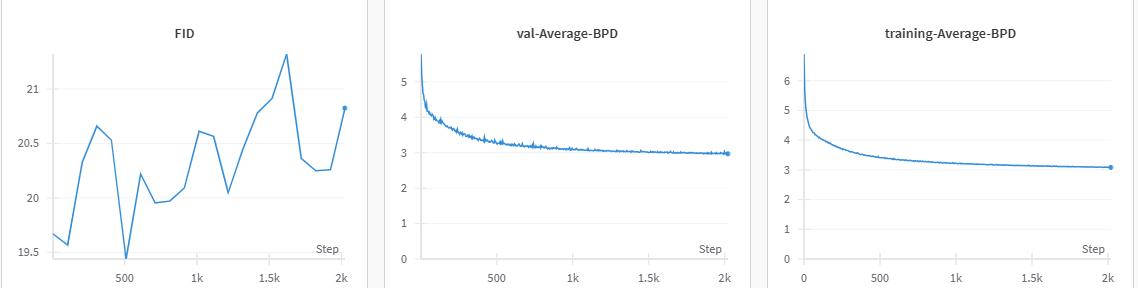
\includegraphics[width=1.0\textwidth]{report_data/o-train.png}
    \caption{ Training curve for the main model.}
    \label{fig:o-train}
  \end{figure}

  \begin{figure}
    \centering
    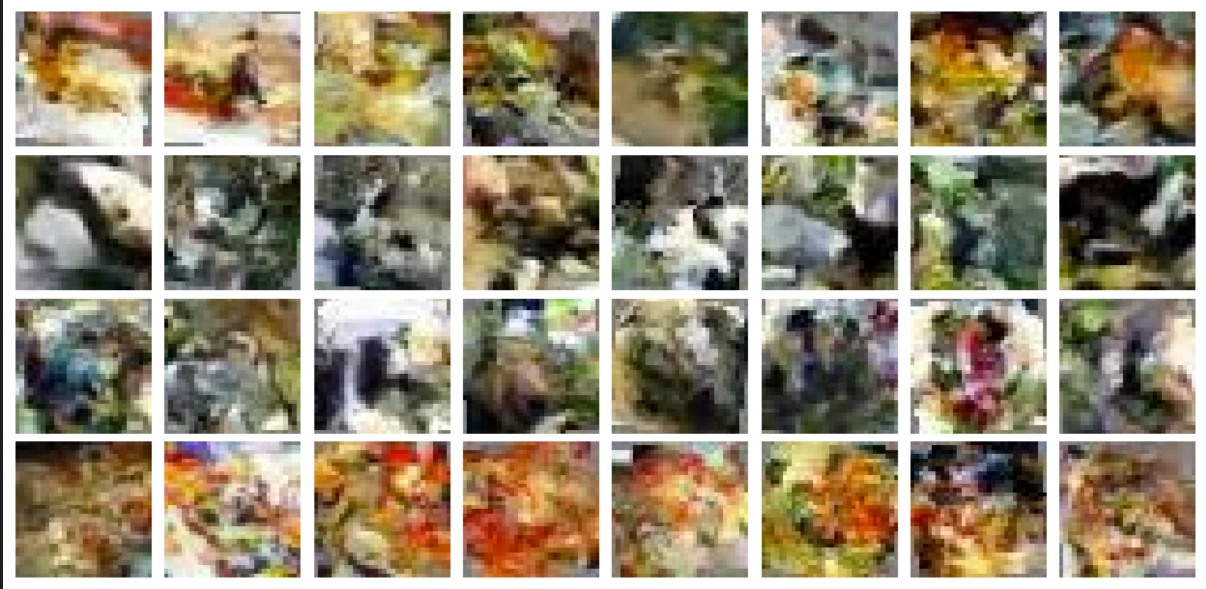
\includegraphics[width=0.9\textwidth]{report_data/o-images.png}
    \caption{ Sample images generated by the model, each row represents a class.}
    \label{fig:o-sample}
  \end{figure}

\subsection{major hyperparameter}
\begin{verbatim}
--batch_size 32 `
--nr_resnet 1 `
--nr_filters 128 `
--nr_logistic_mix 100 `
--lr_decay 0.99995 `    # until batch 501, changed to 0.997 afterward 
--lr 0.0002 `           # until batch 501, changed to 0.0001 afterward
--max_epochs 801 `      # final batch used is 775, however, validation accuracy reached 86+ since batch 300
--seed 4399
\end{verbatim}

\subsection{Training and setup}
\label{train}
Please reference the appended CPEN455HW-2023W2\textbackslash README\_TECH.md file.

\subsection{Results}
With the model trained, we achieved an accuracy of 0.89\% and f1 of 0.89\% on the test set with a fid score of 21.3, as shown in Figure \ref{fig:o-fid-fin}.

\begin{figure}
    \centering
    
\includegraphics[width=0.5\textwidth]{report_data/o-fid-img.png}
    \caption{ FID score of generated image (100) }
    \label{fig:o-fid-fin}
  \end{figure}

\subsection{Alternative solutions attempted}
\label{alternative_solution}


We explored several interesting alternative solutions, detailed below, which did not yield as promising results as our chosen approach. Unless stated otherwise, all models were trained with the hyperparameters [resnet = 1, filter = 40, logistical\_mix = 10] for 200 epochs without fine-tuning. Measured accuracies were taken from the highest performing checkpoints. For context, our reduced parameter model achieved an accuracy of 74.1\% on the validation dataset at epoch 200 with a Fréchet Inception Distance (FID) of 37.6, increasing to 81.2\% accuracy and a FID of 28.7 at epoch 350 (the optimal point within a 500 epoch span).

\begin{itemize}
    \item Specialized preprocessing techniques, such as image segmentation, swapping, noise, and data masking, did not enhance the training or fine-tuning performance of the model. These methods may not have been effective due to the limited training data and PixelCNN's pixel-wise generation characteristic. Validation accuracy decreased from 74.1\% to 73.3%.
    \item Employing a Polyak Averaged Model, integrated at the ResNet block level, showed potential in improving FID scores but failed to significantly boost classification accuracy. Validation accuracy peaked at 77.2\% after 450 epochs.
    \item A complete structural overhaul to include a label channel was unsuccessful in elevating classification accuracy beyond mere random chance. Generated images from this model failed to resemble input images, indicating possible structural or implementation errors. Optimal validation accuracy was a mere 25.2\% over 400 epochs, with 28.7 FID at the same checkpoint.
    \item Modifying the PCNN++G by eliminating the final addition with the input matrix in favor of purely relying on convolution layers resulted in a reasonable FID of 25.5 at epoch 200, but a disappointing classification accuracy of only 69.2\%. This is the approach utilized by vann den Oord et al. [2] in third approach to conditional PIXELCNN model. However, the highlighted approach utilized additional conditional AVE decoder which was not implemented by this solution.
    \item Revising PixelCNNLayer\_up/down and ResNet to introduce a new set of weights at each layer, which are multiplied by the class label embedding prior to convolution, demonstrated a stronger correlation between image components and their classification at every layer. This approach reached an accuracy of 84.9\% at epoch 300 but exhibited signs of increasing BPD due to the handling of gradients. The BPD curve for this model variation is shown in Figure \ref{fig:F-BPD}.
    \item Eliminating specific label dependencies in favor of a single weight matrix interacting with the labels resulted in no overfitting, achieving a validation accuracy of 71.8\% at epoch 500, with occasional sub-20 FID scores. However, this model struggled to generalize effectively to the test dataset at high parameter settings, achieving a test accuracy of 86.1\% by epoch 475 (increasing to 87.6\% post-fine-tuning). A comparison with our proposed model is illustrated in Figure \ref{fig:F-pp_cmp}.
    \item For further details on classification, fine-tuning, data analysis, and training processes, please refer to the technical documentation detailed in \ref{train}.
\end{itemize}

\begin{table}
    \caption{Model Performance Comparison}
    \label{model_cmp}
    \centering
    \begin{tabular}{llll}
      \toprule
      Model Variant & Epoch & Validation Accuracy (\%) & FID \\
      \midrule
      PIXELCNN++G   & 350 & 74.1 & 28.7 \\
      PIXELCNN++G   & 350 & 81.2 & 28.7 \\
      Polyak Averaged Model     & 200 & 77.2 & - \\
      Label Channel Model       & 400 & 25.2 & - \\
      Pure Convolution          & 200 & 69.2 & 25.5 \\
      Modified PixelCNNLayer    & 300 & 84.9 & - \\
      Single Weight Matrix      & 500 & 71.8 & <20 \\
      \bottomrule
    \end{tabular}
\end{table}

\begin{figure}
    \centering
    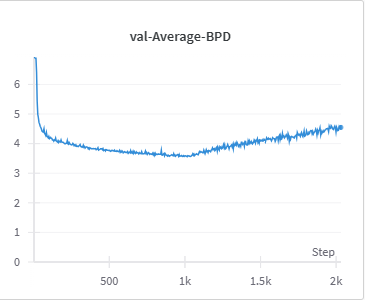
\includegraphics[width=0.5\textwidth]{report_data/f_2_BPD.png}
    \caption{BPD curve for the model with new set of weights at every layer.}
    \label{fig:F-BPD}
  \end{figure}

  \begin{figure}
    \centering
    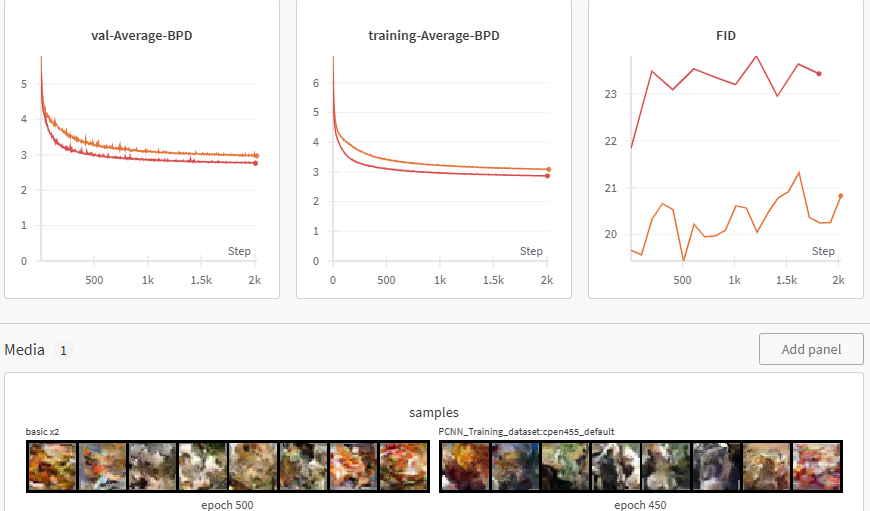
\includegraphics[width=0.5\textwidth]{report_data/f_pp_cmp.png}
    \caption{Comparison between the final model and the model with different down-sampling weights for each class.}
    \label{fig:F-pp_cmp}
  \end{figure}

\section{Conclusion}

In conclusion, with the modifications from the author, the PixelCNN++G model was able to achieve a classification accuracy of 88.9\% on the tes dataset, with a FID score of 21.3. The model and corresponding code is included as appendix to this report.


\section{Supplementary Material}

\subsection{GPT-Use}
Sections of the code modified by GPT is labeled in line with comment. One can find the chat history with GPT in the supplementary materials section

\begin{figure}[H]
    \centering
    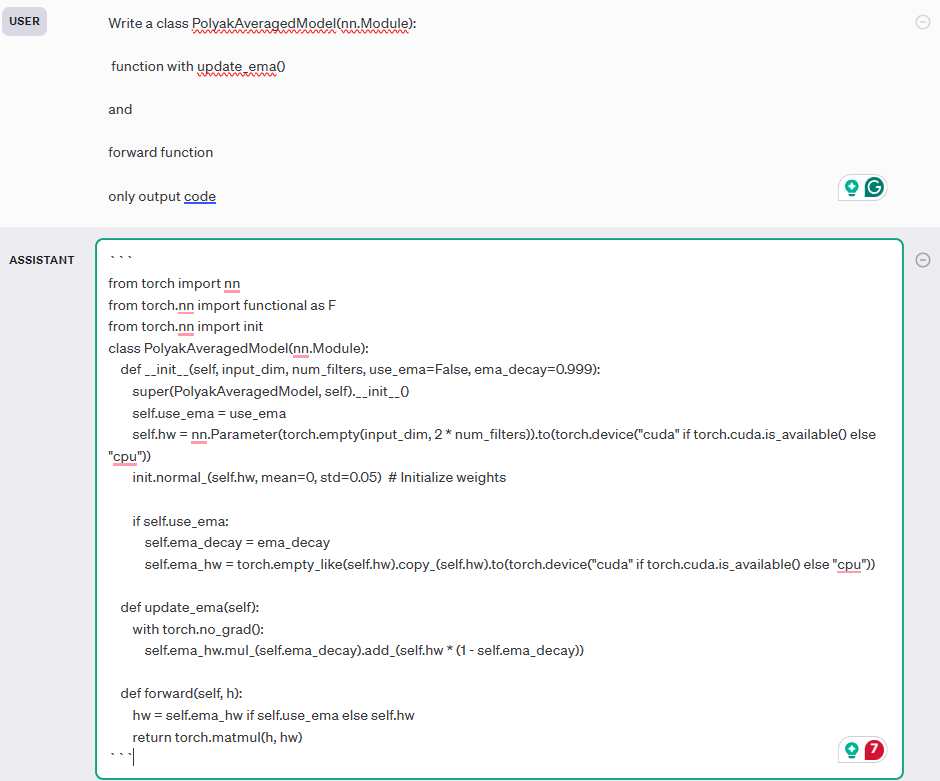
\includegraphics[width=0.5\textwidth]{report_data/g-1.png}
\end{figure}

\begin{figure}[H]
    \centering
    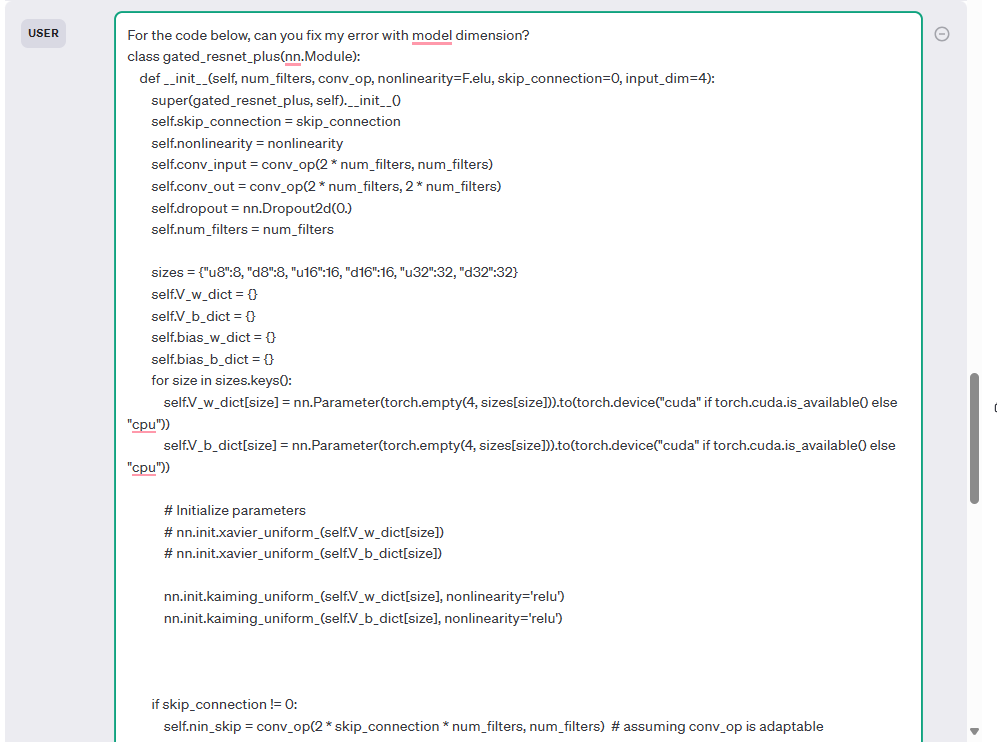
\includegraphics[width=0.5\textwidth]{report_data/g-2.png}
\end{figure}

\begin{figure}[H]
    \centering
    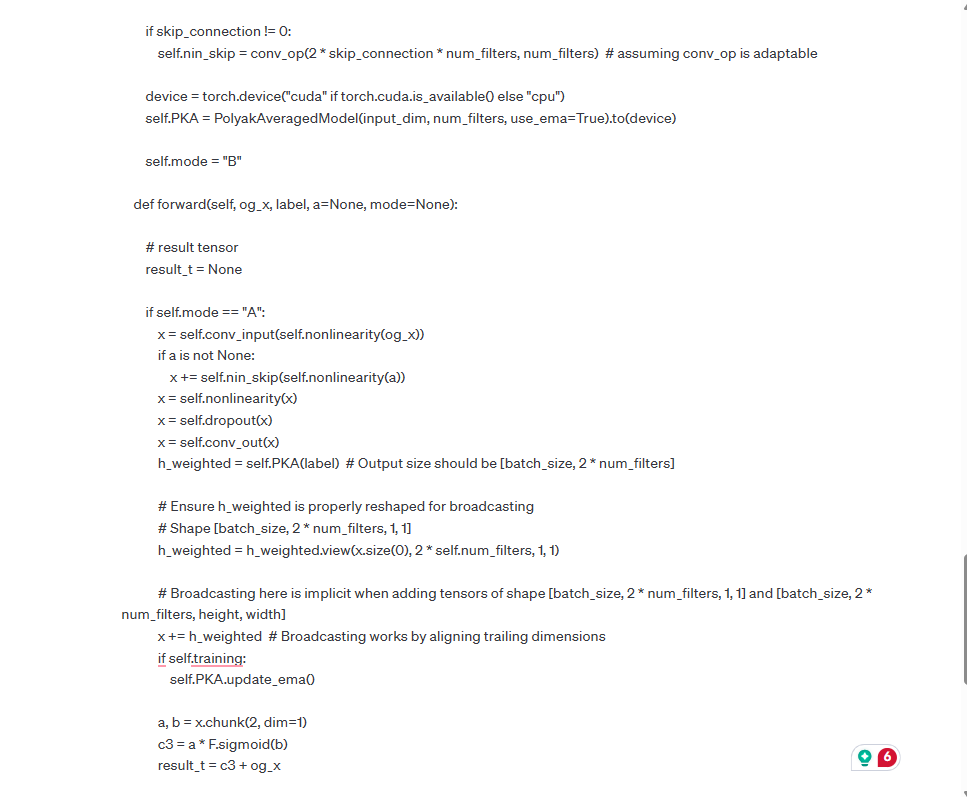
\includegraphics[width=0.5\textwidth]{report_data/g-3.png}

\end{figure}

\begin{figure}[H]
    \centering
    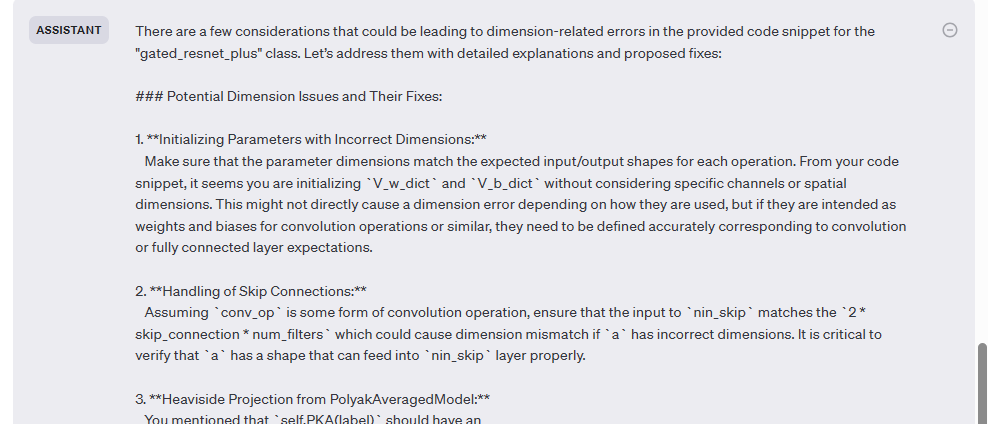
\includegraphics[width=0.5\textwidth]{report_data/g-4.png}
\end{figure}

\begin{figure}[H]
    \centering
    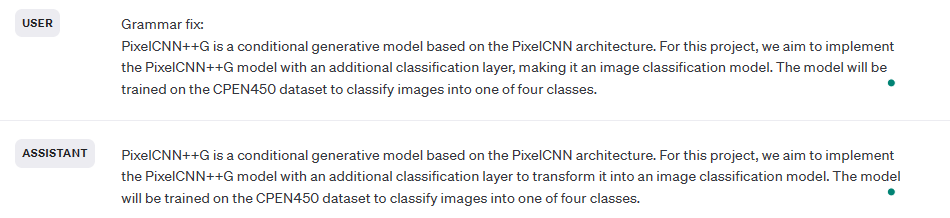
\includegraphics[width=0.5\textwidth]{report_data/g-5.png}
\end{figure}

\begin{figure}[H]
    \centering
    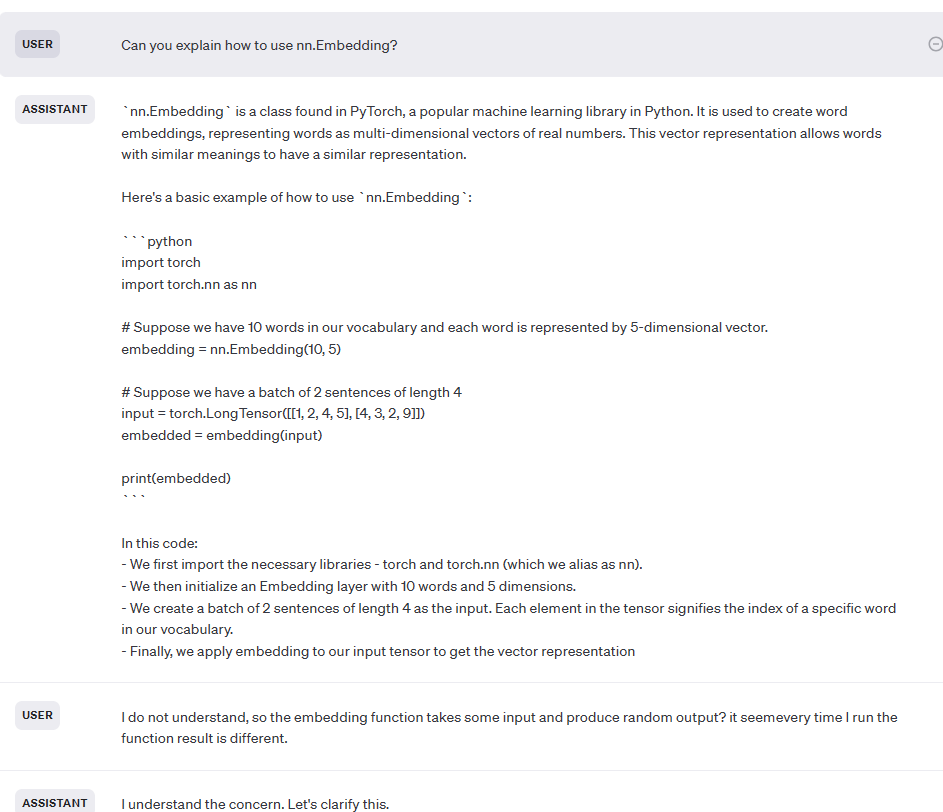
\includegraphics[width=0.5\textwidth]{report_data/g-6.png}
\end{figure}

\begin{figure}[H]
    \centering
    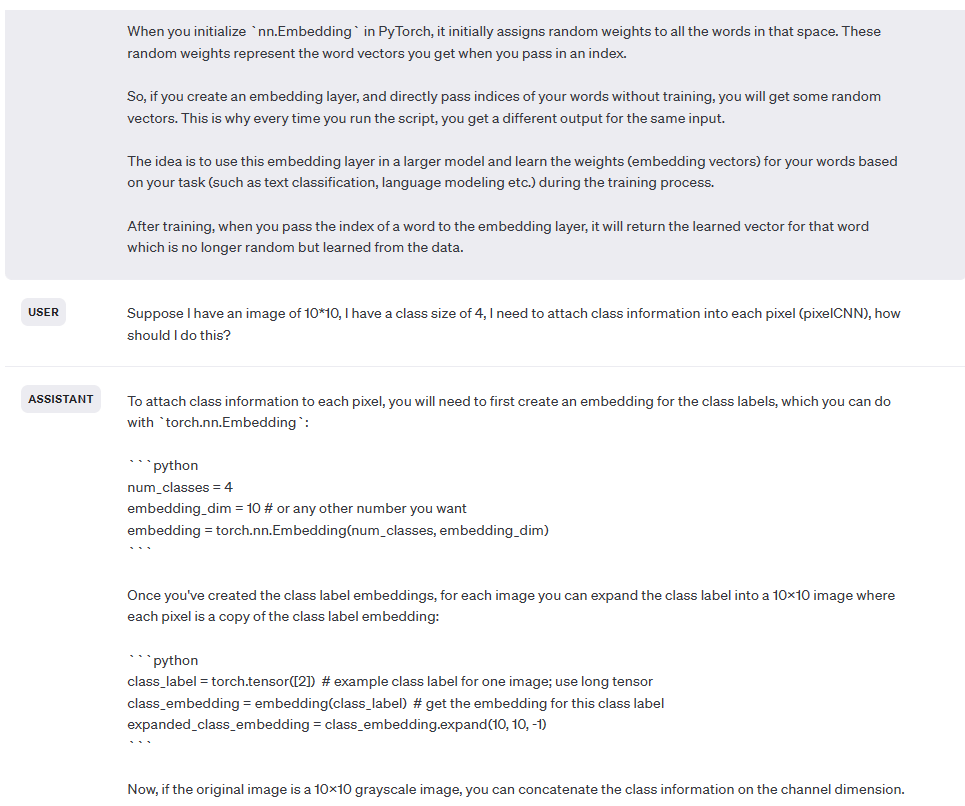
\includegraphics[width=0.5\textwidth]{report_data/g-7.png}
\end{figure}

\begin{figure}[H]
    \centering
    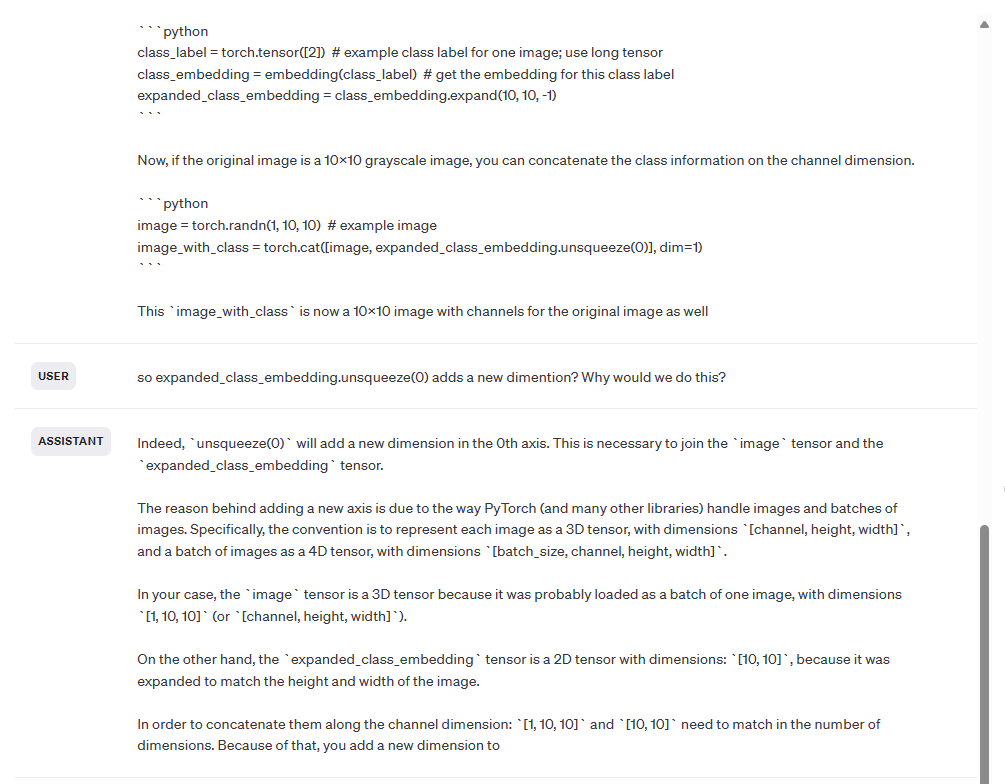
\includegraphics[width=0.5\textwidth]{report_data/g-8.png}
\end{figure}

\begin{figure}[H]
    \centering
    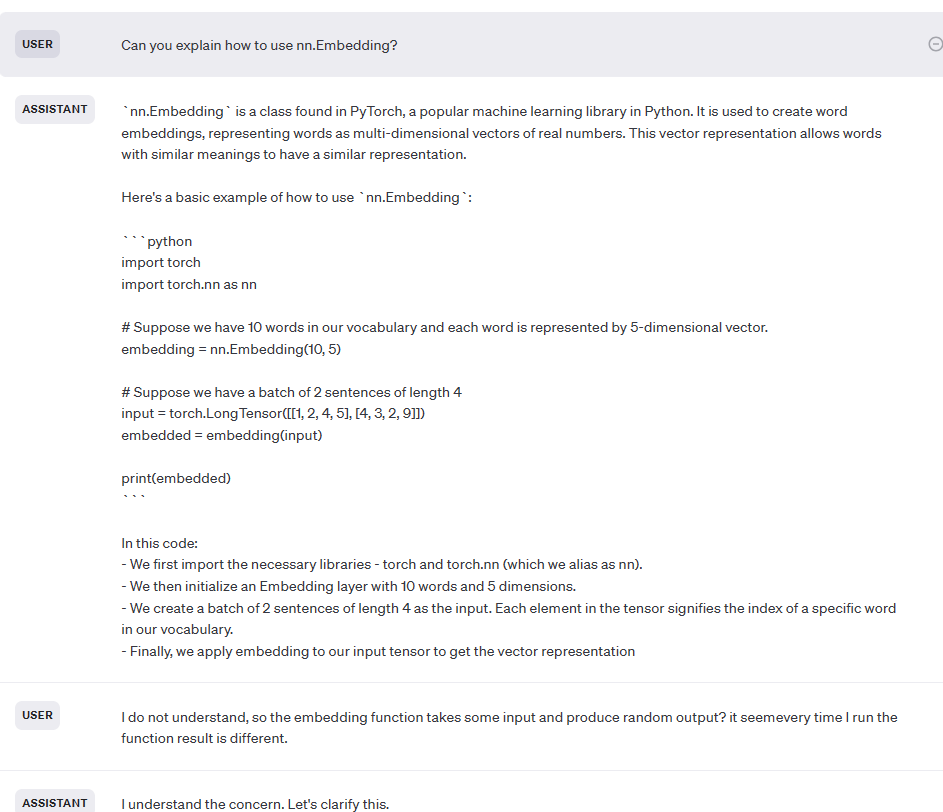
\includegraphics[width=0.5\textwidth]{report_data/g-9.png}
\end{figure}

\begin{figure}[H]
    \centering
    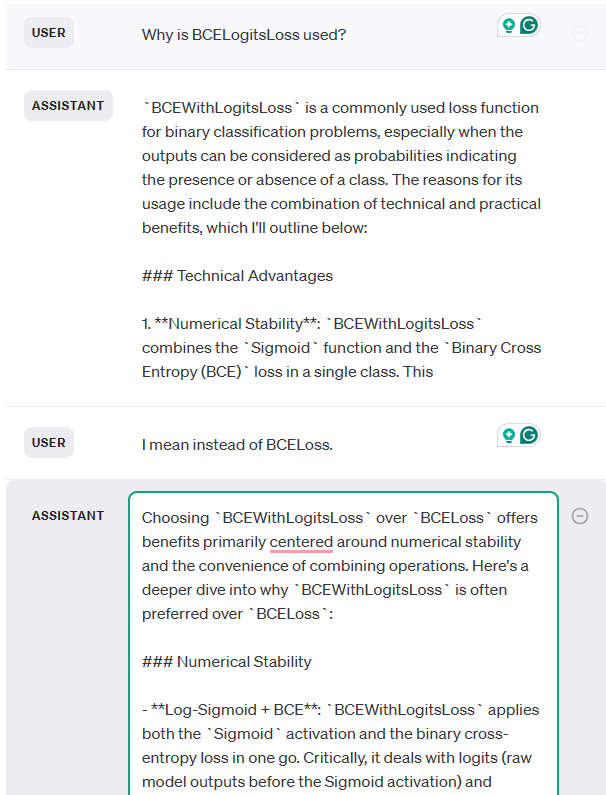
\includegraphics[width=0.5\textwidth]{report_data/g-10.png}
\end{figure}

\begin{figure}[H]
    \centering
    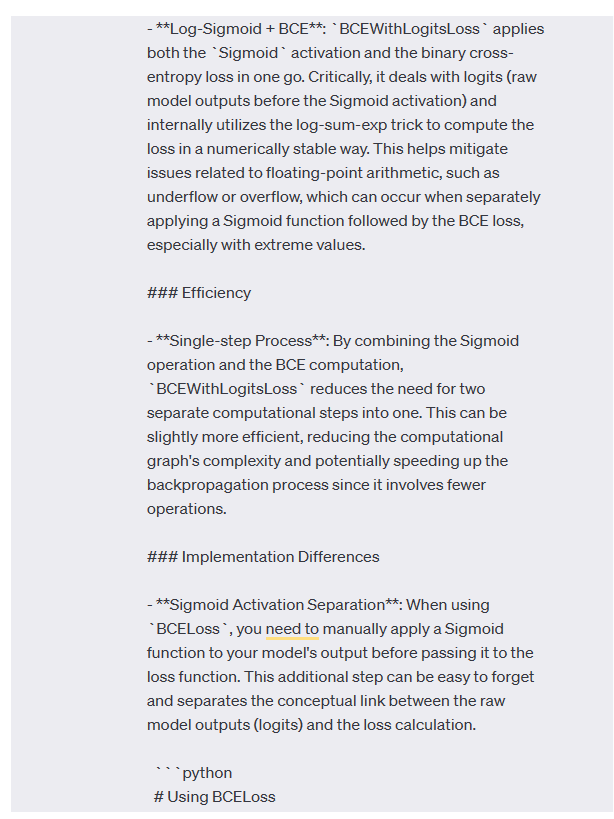
\includegraphics[width=0.5\textwidth]{report_data/g-11.png}
\end{figure}

\begin{figure}[H]
    \centering
    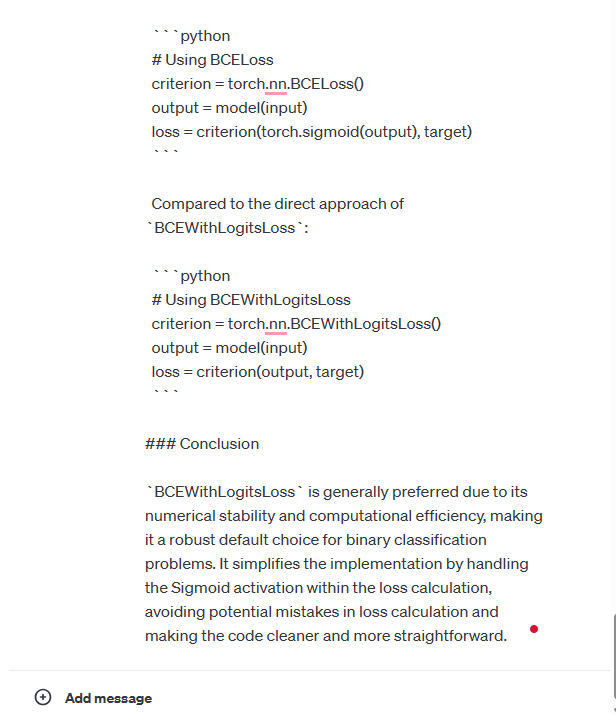
\includegraphics[width=0.5\textwidth]{report_data/g-12.png}
\end{figure}

\begin{figure}[H]
    \centering
    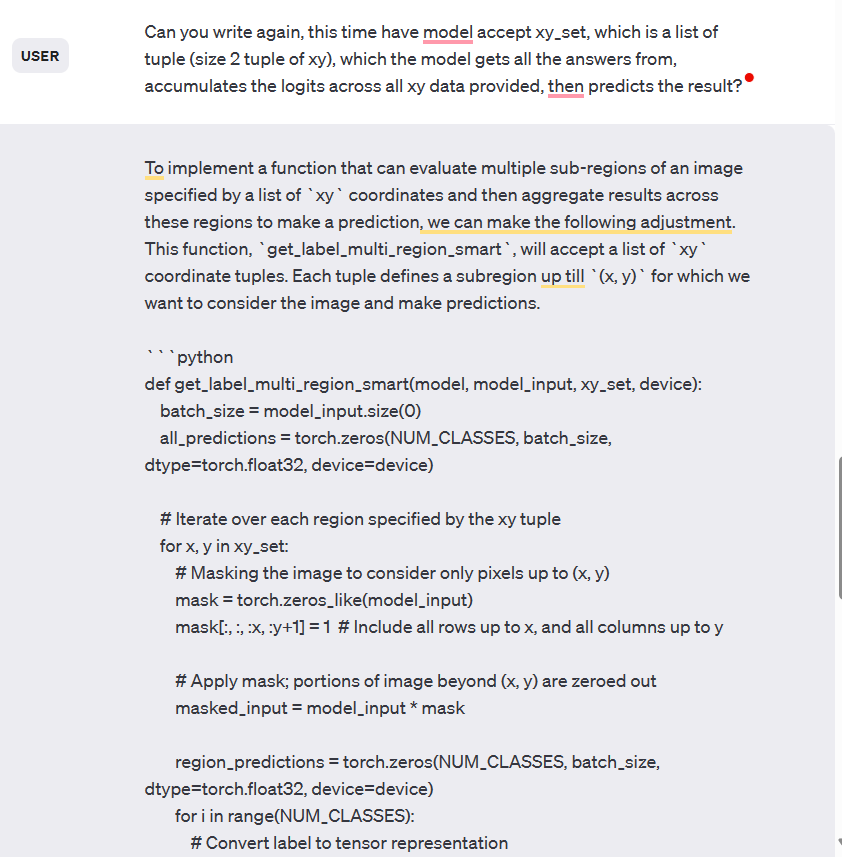
\includegraphics[width=0.5\textwidth]{report_data/g-13.png}

\end{figure}

\begin{figure}[H]
    \centering
    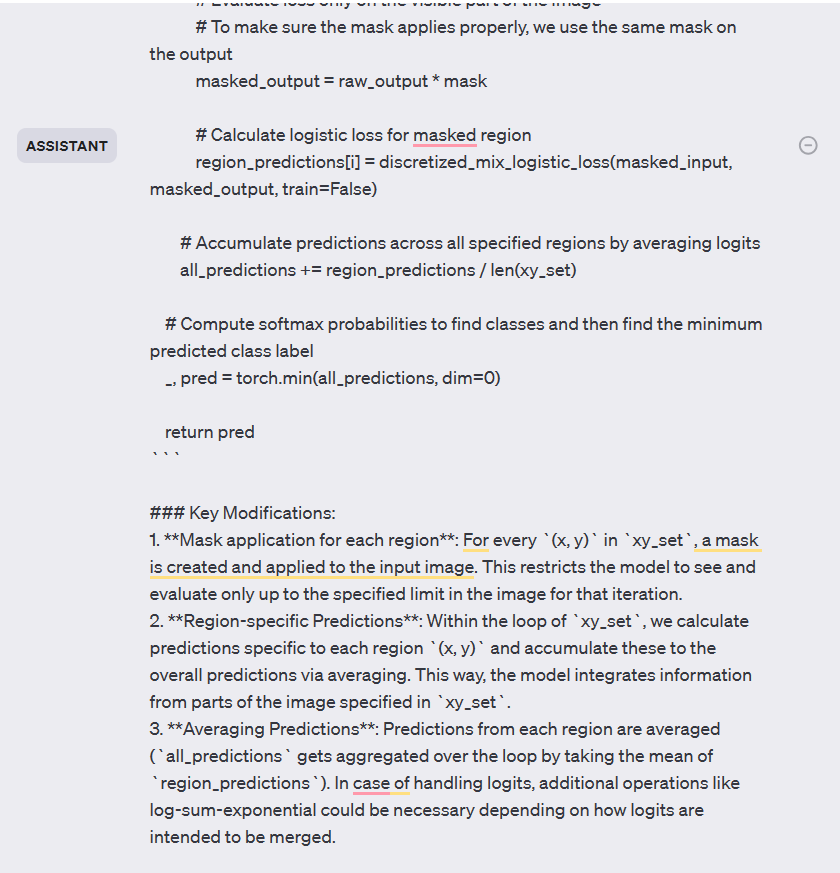
\includegraphics[width=0.5\textwidth]{report_data/g-14.png}
\end{figure}

\begin{figure}[H]
    \centering
    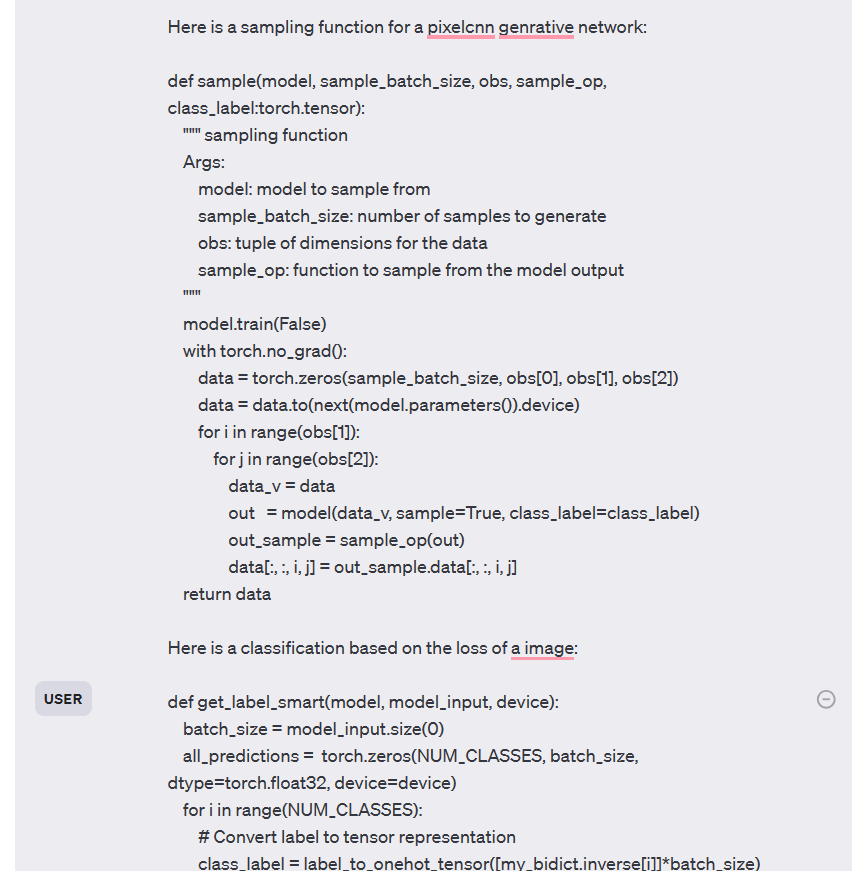
\includegraphics[width=0.5\textwidth]{report_data/g-14_.png}
\end{figure}

\begin{figure}[H]
    \centering
    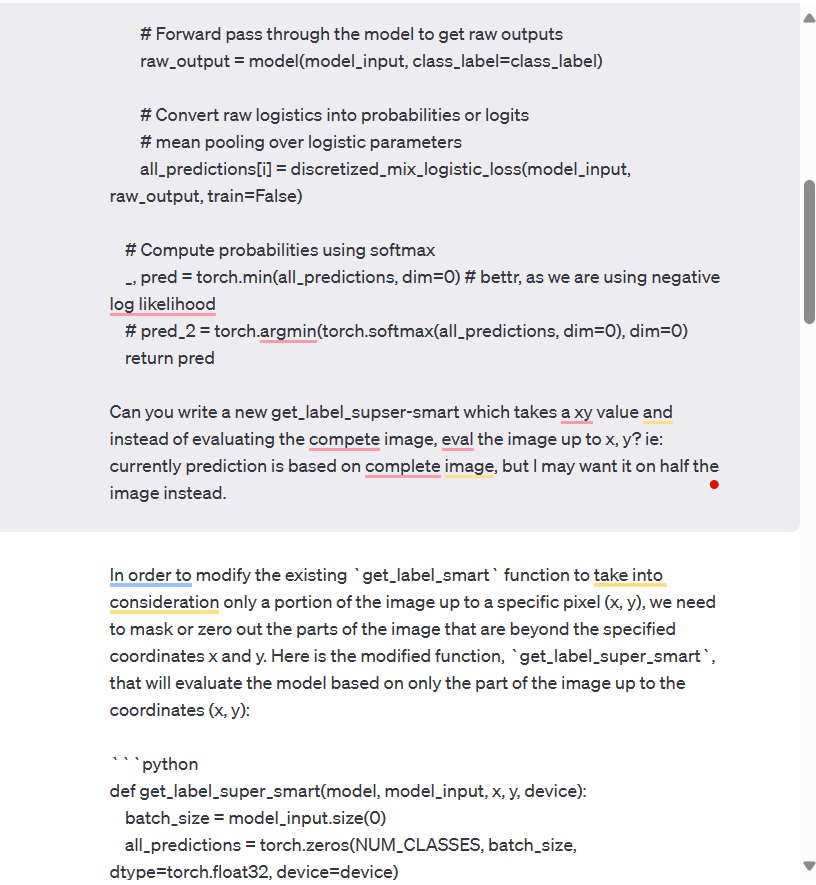
\includegraphics[width=0.5\textwidth]{report_data/g-15.png}
\end{figure}

\begin{figure}[H]
    \centering
    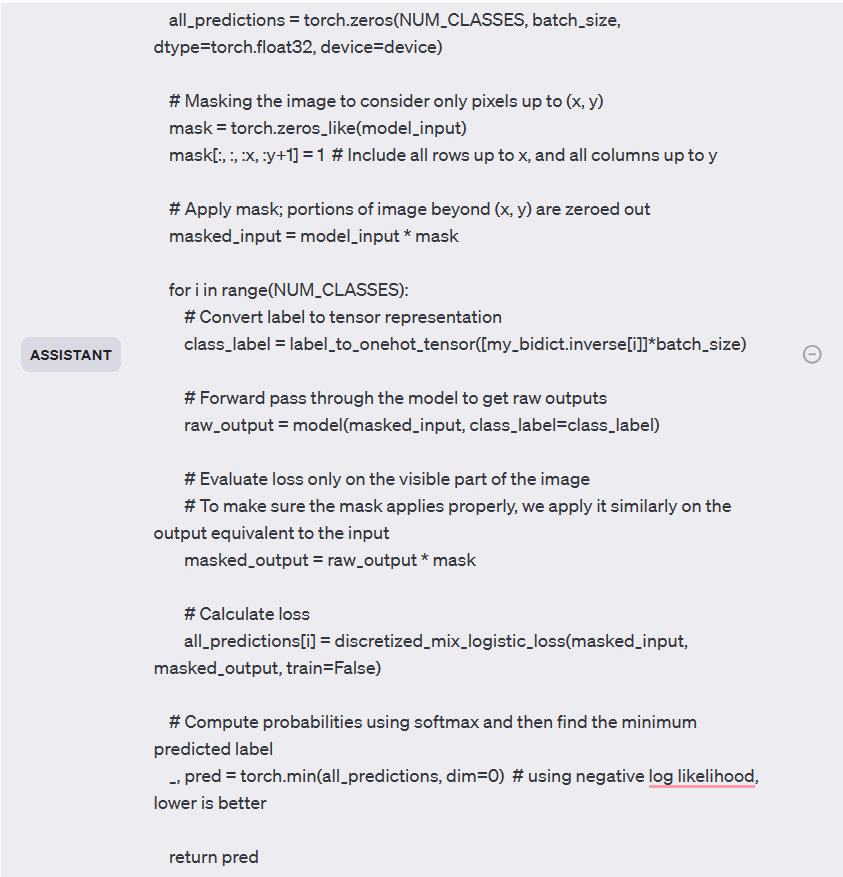
\includegraphics[width=0.5\textwidth]{report_data/g-16.png}
\end{figure}

\begin{figure}[H]
    \centering
    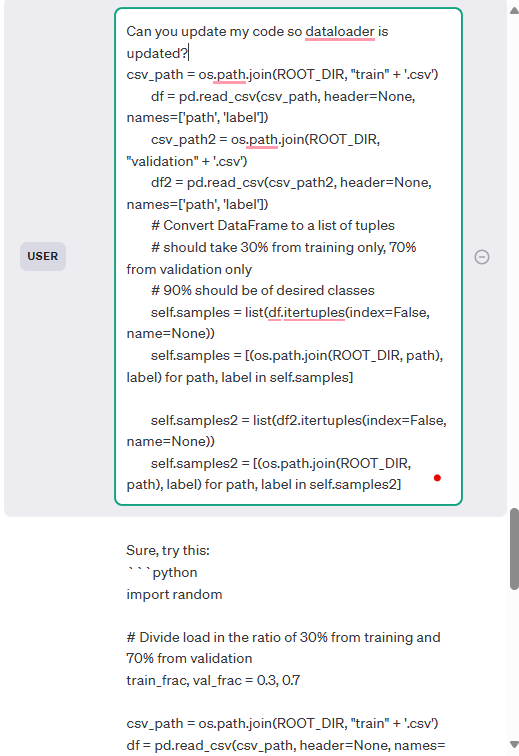
\includegraphics[width=0.5\textwidth]{report_data/g-17.png}
\end{figure}

\begin{figure}[H]
    \centering
    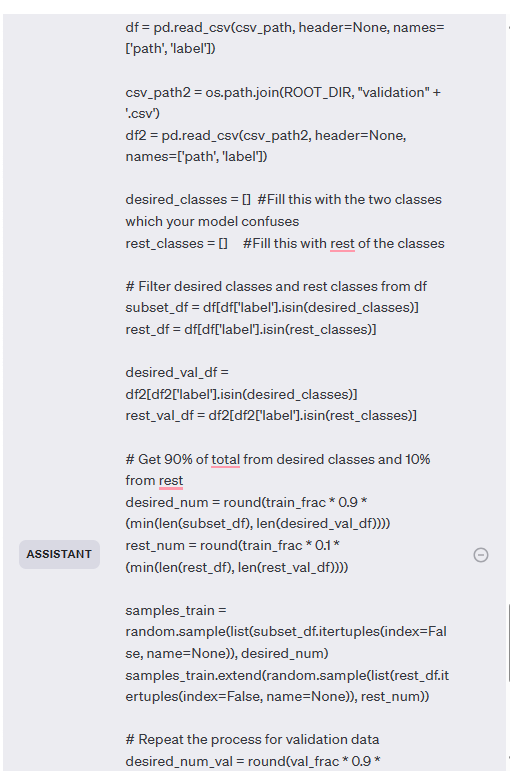
\includegraphics[width=0.5\textwidth]{report_data/g-18.png}
\end{figure}

\begin{figure}[H]
    \centering
    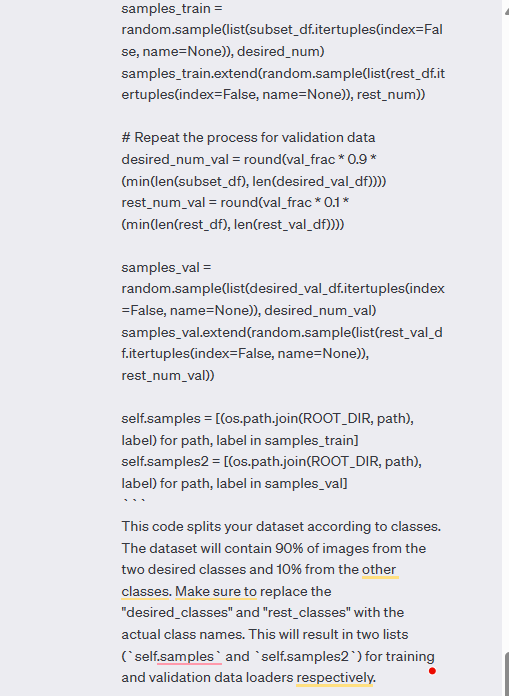
\includegraphics[width=0.5\textwidth]{report_data/g-19.png}
\end{figure}



\section*{References}
% base
[1] T. van den Salimans, A. Karpathy, X. Chen, and D. p. Kingma, PIXELCNN++: IMPROVING THE PIXELCNN WITH DISCRETIZED LOGISTIC MIXTURE LIKELIHOOD AND OTHER MODIFICATIONS, 2017. Accessed: 2024. [Online]. Available: https://arxiv.org/pdf/1606.05328.pdf

% simple 
[2] A. van den Oord et al., Conditional Image Generation with PixelCNN Decoders, 2016. Accessed: 2024. [Online]. Available: https://arxiv.org/pdf/1606.05328.pdf

\end{document}